%% Pure Rho and Cost: one authored calculus, named extensions, corrected hypotheses
%%
%% Build:
%%   pdflatex rho.tex

\documentclass[11pt]{article}
\usepackage[T1]{fontenc}
\usepackage[utf8]{inputenc}
\usepackage{lmodern}
\usepackage{geometry}
\geometry{margin=1in}
\usepackage{hyperref}
\usepackage{booktabs}
\usepackage{tabularx}
\usepackage{amsmath}
\usepackage{amssymb}
\usepackage{tikz}
\usetikzlibrary{arrows.meta,positioning}
\usepackage{listings}
\setlength{\emergencystretch}{3em}
\lstset{
  basicstyle=\ttfamily\small,
  breaklines=true,
  frame=single,
  columns=fullflexible
}
\newcommand{\leanfile}[2]{\href{https://github.com/zariuq/MeTTapedia/blob/main/lean/mettapedia/Mettapedia/#1}{\code{#2}}}

\newcommand{\code}[1]{\texttt{#1}}
\newcommand{\formalized}{\textbf{[formalized]}}
\newcommand{\open}{\textbf{[open]}}
\newcommand{\refuted}{\textbf{[counterexample recorded]}}

\title{Pure Rho and Cost:\\
One Authored Calculus, Named Extensions, and Corrected Hypotheses}
\author{Mettapedia}
\date{July 2026 (working paper)}

\begin{document}
\maketitle

\begin{abstract}
The rho-calculus is a process calculus in which every name is a quoted
process. This paper fixes the exact calculus we formalize and implement: a
\emph{pure core} whose only operational reduction is communication, with
every engine convenience recorded as a named extension derived from that
core, never mixed into it. On this base we state the cost construction ---
wrapping terms and gating reductions by funding --- together with two
corrections to its published hypotheses: the injectivity assumption behind
\emph{quote-faithfulness} cannot hold for ordinary monad multiplication on
any nontrivial signature monoid: joint injectivity of multiplication together
with a two-sided unit forces the carrier to be a subsingleton.  The repair is
not a stronger monoid hypothesis.  Funded execution instead forms an
Atkey-style parameterized monad indexed by complete pre- and post-resource
states.  Exact causal receipts are retained for authority decisions, while
prices and budget totals factor through explicit, generally non-injective
aggregation maps.  The obstruction, the parameterized monad laws, this
authority/observation factorization, and a computable canonical section for
pure structural congruence are formalized.  Beyond the single calculus, Cost
is developed as a construction on \emph{continued interactive GSLTs} ---
languages equipped with one ordered interaction cut, a computable canonical
section, and a position-sensitive continuation-retyping plan --- and the
generated funded language is itself such an object, with the object-closure
laws of the resulting endofunctor programme largely discharged.  A second
compiled counterexample is recorded: the global raw fiber-stability
hypothesis of our earlier normalization architecture is false for rho, and
its repair moves the entire equational theory onto typed open carriers with
proof-relevant elaboration, on which exact canonical laws cut out the full
subcategory hosting strict $\mathrm{Cost}_1$.  Public raw admission checks
both the cost grammar and whole-object binder scope, including purse
locations.  On that admitted fragment, the budgeted Lean executor refines a
declarative funded trace and erases to a path of the pure-rho GSLT
mechanically derived from the authored language definition, with exactly one
COMM step per funded event.  Claims are marked as formalized or open;
nothing here is asserted beyond its marker.
\end{abstract}

\section{Introduction}

A calculus and its implementation drift apart unless the boundary between
them is a maintained artifact. Reference implementations of the
rho-calculus add conveniences --- direct execution of quoted processes,
polyadic inputs, name extrusion --- that are individually reasonable and
collectively fatal to the question ``what exactly has been proved?''
Our answer is architectural:

\begin{center}
\resizebox{0.98\linewidth}{!}{%
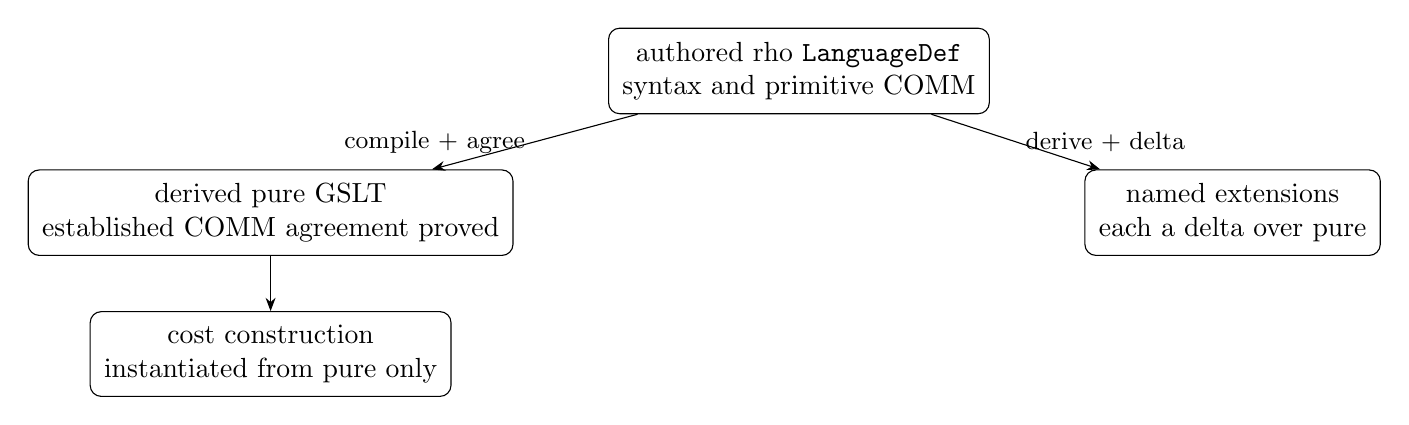
\begin{tikzpicture}[node distance=7mm and 12mm,
  box/.style={draw, rounded corners, align=center, inner sep=5pt}]
\node[box] (root) {authored rho \code{LanguageDef}\\syntax and primitive COMM};
\node[box, below left=of root] (pure) {derived pure GSLT\\established COMM agreement proved};
\node[box, below right=of root] (ext) {named extensions\\each a delta over pure};
\node[box, below=of pure] (cost) {cost construction\\instantiated from pure only};
\draw[-{Stealth}] (root) -- (pure) node[midway,left,font=\small]{compile + agree};
\draw[-{Stealth}] (root) -- (ext) node[midway,right,font=\small]{derive $+$ delta};
\draw[-{Stealth}] (pure) -- (cost);
\end{tikzpicture}
}
\end{center}

The authored \code{LanguageDef} is the intended source presentation for the
strict syntax and primitive COMM rule.  The present Lean development proves
that its compiled matcher, normalization, substitution, and supported COMM
contracta agree with the independently established semantic development.  The
pure GSLT used below is itself derived from that authored declaration, so the
agreement theorem does not create a second operational authority.  Named
extensions import the pure theory and add explicit deltas; the pure theory and
the runtime cost profile import none of them.  Full equivalence between the
complete derived contextual relation and the independently established
relation is a separate theorem obligation, not assumed here.

\section{The pure calculus}

\paragraph{Syntax.} Processes $P$ and names $x$ are mutually defined:
\[
P \;::=\; 0 \;\mid\; \mathsf{for}(y \leftarrow x)\,P \;\mid\; x!(P)
 \;\mid\; P \,|\, P \;\mid\; {*}x
\qquad\qquad
x \;::=\; @P .
\]
A name is a quoted process $@P$; the process ${*}x$ is the \emph{drop} of
a name. Quotation and dropping are the calculus's reflection: processes
can be passed as data and data can be run --- but, as we now make precise,
only through communication.

\paragraph{Two equivalences, kept separate.} The calculus has two
distinct static equivalences, and sorting laws into the correct one is
load-bearing:
\begin{itemize}
\item \emph{Name equivalence} contains the cancellation
  $@({*}x) \equiv_N x$: quoting the drop of a name gives back the name.
  This is an equation between \emph{names}.
\item \emph{Process structural congruence} contains
  alpha-equivalence and the commutative-monoid laws for parallel
  composition ($P|Q \equiv Q|P$, $(P|Q)|R \equiv P|(Q|R)$, $P|0 \equiv P$).
\end{itemize}
Neither equivalence contains a rule that \emph{runs} anything.
In particular, ${*}(@P) \to P$ is \emph{not} a law of the pure calculus,
neither as an equation nor as a reduction.

\paragraph{One reduction.} The only operational rule is communication:
\[
\mathsf{for}(y \leftarrow x)\,P \;\big|\; x!(Q)
\;\longrightarrow\;
P\{@Q/y\},
\]
where the substitution is semantic: when $P\{@Q/y\}$ replaces $y$ inside a
drop, ${*}y$ becomes $Q$. Dequotation therefore happens \emph{only}
through substitution after a communication --- you can run exactly the
code you were sent.

\paragraph{A positive and a negative example.}
\[
\underbrace{\mathsf{for}(y \leftarrow @0)\,({*}y)
\;\big|\; @0!(x!(0))}_{\text{reducible}}
\;\longrightarrow\; x!(0)
\qquad\qquad
\underbrace{{*}(@\,x!(0))}_{\text{stuck in pure rho}}
\;\not\longrightarrow
\]
The left process communicates on the name $@0$ and the received quoted
process runs via substitution. The right process is a free-standing drop
of a quotation; in the pure calculus it is inert. \formalized{} for the
concrete one-step relation (communication is its only constructor);
the corresponding negative example is part of the extension test suite
described in Section~\ref{sec:ext}.

\section{Running quoted code without extending the calculus}
\label{sec:runner}

The convenience that tempts implementations to add a primitive
${*}(@P) \to P$ step is already expressible, at the cost of one honest
communication, by a two-process \emph{runner} idiom:
\[
\mathit{run}!(@P) \;\big|\; \mathsf{for}(y \leftarrow \mathit{run})\,({*}y)
\;\longrightarrow\; P .
\]
The drop fires through substitution on a received name --- pure rho ---
and the execution of a quoted process costs exactly one communication
event, which the cost semantics of Section~\ref{sec:cost} meters
honestly. Nothing about expressivity forces an execution primitive into
the calculus; adding one changes the step relation, the stuck states,
and every cost ledger, in exchange for saving a single COMM.

\section{Extensions as named deltas}
\label{sec:ext}

Engine conveniences are legitimate --- as \emph{named} extensions.
The discipline has three parts.

\paragraph{Structure.} Each extension is a delta over the pure theory:
the extension module imports the pure calculus and adds constructors,
equations, or rules; the pure modules import no extension. Distinct
conveniences are distinct deltas --- at minimum, a minimal
\emph{execution} extension (pure rho plus ${*}(@P) \to P$) is kept
separate from a \emph{reference-implementation profile} (polyadic input,
replicated input, name extrusion, native data operations), because they
change different parts of the theory and generate different cost events.
In the formal library these deltas may be collected in one clearly
labelled extended-rho namespace; the runtime's cost profile instantiates
none of them.

\paragraph{Theorems, not conventions.} Each delta carries a positive and
a negative theorem: the free drop \emph{cannot} step in pure rho
\formalized{}; the free drop \emph{does} step in the execution extension
\formalized{}; and the cost profile is instantiated from the pure calculus
specifically. The two reduction claims are proved for the declarative language
definitions.  The runtime import/profile boundary remains a separate closure
gate. A text search for stray constructors is useful supplementary evidence;
the load-bearing boundary is the import graph and these theorems.

\paragraph{The delta as a document.} A reference implementation's
distance from the paper calculus is itself worth recording. The audit of
the implementation we compare against (the \code{mettail} engine's rho
language) yields exactly such a delta: an execution rewrite, polyadic and
persistent communication, extrusion, and native data --- all useful, none
of them part of the calculus whose metatheory we prove. Recording the
delta turns ``the paper and the code disagree'' from folklore into data.

\section{The cost construction: corrected hypotheses}
\label{sec:cost}

The cost construction wraps terms and gates reduction by funding: a
wrapped redex fires only when the wrapper supplies a token drawn from a
commutative monoid $(S, *, e)$ of \emph{signatures}, and each reduction
consumes its funding and emits a receipt. Runtime aspects --- receipts,
budgets, parallel execution --- are treated in the companion engine
paper; here we state the mathematical hypotheses, two of which require
correction.

\subsection{The quote-faithfulness obstruction}

Call a map \emph{quote-faithful} when it is injective on the signature
keys reachable in a given theory. The published development uses
per-argument injectivity of the signature operation. Three separate
claims hide under this phrase, with three different fates.

\paragraph{(a) Fixed-element level.} ``Multiplication by a fixed $s$ is
injective'' ($s * a = s * b \Rightarrow a = b$) is exactly
\emph{cancellativity} of the monoid --- and it \emph{fails} in general:
\[
\max(3, 1) = \max(3, 2)
\qquad\qquad
\infty + 1 = \infty + 2 .
\]
Idempotent (tropical) aggregation and saturating budgets are therefore
outside the hypothesis. Free signatures --- finite multisets of
generators --- are cancellative, so the intended examples survive
\emph{at this fixed-element level once the hypothesis is stated}.
\formalized{}

\paragraph{(b) Multiplication level.} The monad multiplication
$\mu : \mathrm{Cost}^2 \to \mathrm{Cost}$ flattens two layers of
wrapping, combining an outer and an inner signature into one key.
Cancellativity does \emph{not} make this flattening injective, because
joint injectivity of $(a,b) \mapsto a * b$ is a unique-factorization
property, not a cancellation property:
\[
1 + 2 \;=\; 0 + 3 \quad\text{in } (\mathbb{N}, +),
\qquad\qquad
\{a\} \uplus \{b, c\} \;=\; \{a, b\} \uplus \{c\}
\quad\text{for free multisets.}
\]
Both monoids are cancellative; in both, distinct outer/inner
factorizations flatten to the same key.  More generally, if a binary
operation with a two-sided unit were jointly injective, then
$(e,a)=(a,e)$ for every $a$, forcing every element to equal $e$.  Thus:
\[
  \operatorname{inj}\bigl((a,b)\mapsto a*b\bigr)
  \quad\Longleftrightarrow\quad
  S\text{ is a subsingleton}.
\]
No nontrivial monoid---including words, free multisets, or natural-number
costs---can satisfy the published multiplication-level requirement.  This is
an impossibility theorem, not a missing hypothesis. \formalized{}

The same obstruction is forced directly by the monad unit laws:
$\mu\circ\eta_{TX}=\mathrm{id}_{TX}=\mu\circ T\eta_X$.  For a nontrivial
grade, the outer-unit and inner-unit placements are distinct factorizations
with the same flattened image.  Thus changing the signature carrier cannot
restore injectivity of ordinary monad multiplication.

\paragraph{(c) Unit level.} The unit $\eta$ must not fabricate funding.
In the corrected semantics, unit is the empty execution at a fixed resource
state and carries the empty receipt.  Every nonempty funded execution advances
the event counter; hence no nonempty execution can masquerade as an identity.
The ordinary ``freely available unit token'' argument is withdrawn.
\formalized{} for the concrete funded semantics.

\subsection{The typed repair: pre/post indexed execution}

Let $I$ be the type of complete funded states: event counter, live resource
components, provenance, and the proofs required to continue safely.  For
$i,j\in I$, let $T(i,j,X)$ be the type of funded executions from $i$ to $j$
returning a value in $X$.  The operations are
\[
  \operatorname{pure}_i : X \to T(i,i,X),
  \qquad
  \operatorname{bind} :
    T(i,j,X) \times (X \to T(j,k,Y)) \to T(i,k,Y).
\]
The shared middle index is part of the type.  An execution ending at $j$ cannot
be composed with one beginning at a different resource state; invalid funding
composition is therefore untypeable.  Empty execution supplies
$\operatorname{pure}$, path concatenation supplies bind, and the two unit laws
and associativity are proved from the corresponding path laws.
\formalized{}

This is an Atkey-style parameterized monad~\cite{atkey}.  It is also the
pre/post-state specialization of the broader graded and parametric-effect
perspective~\cite{katsumata,orchard-wadler-eades}: a
monoid grade summarizes effects, while a category grade records which state
transitions may compose.  The present formalization constructs the resource
transition category and the parameterized monad instance; it does not claim a
fully general category-graded monad for arbitrary result families.

\subsection{Authority is exact; pricing is an observation}

A causal receipt retains event occurrences, funding records, and their order.
Sequential composition concatenates these exact receipts.  Budget totals,
additive prices, multiplicative prices, and signature multisets are obtained
only afterward by monoid homomorphisms:
\[
 \mathrm{Receipt}
   \longrightarrow \mathrm{Aggregate}
   \longrightarrow \mathrm{Price}.
\]
The first object is suitable for replay and authority decisions; the later
objects intentionally forget information.  In particular, the raw account
functor is proved to factor through the exact authority-receipt functor and an
explicit aggregation homomorphism.  The aggregation is not injective, and no
total reconstruction from it exists. \formalized{}

\subsection{What stands}

The concrete runtime already follows the corrected shape: it retains receipts,
gates every firing by actual funding, and derives totals by folding.  Its
receipt replay, sequential/threaded agreement, and sanitizer evidence do not
depend on joint injectivity of signature multiplication.  What is withdrawn is
the ordinary-monad faithfulness claim.  What replaces it is stronger where
authority matters: exact indexed transitions and exact receipts, with every
lossy view named as an observation.

\section{The continued category: Cost as a construction on languages}
\label{sec:continued}

The corrected hypotheses of Section~\ref{sec:cost} are stated for one
calculus.  The deeper architectural claim --- Meredith's ``wrapping by
construction'' --- is that Cost is a \emph{construction on languages}: it
should consume a language equipped with one interaction and return another
such language, so that wrapping composes.  Making that precise forced a
new compositional object, and we consider the result one of the genuinely
novel architectures of this development.  This section states it exactly
as formalized.  The staging is a strict tower --- each stage adds one kind
of structure and forgets none:

\begin{center}
\resizebox{0.98\linewidth}{!}{%
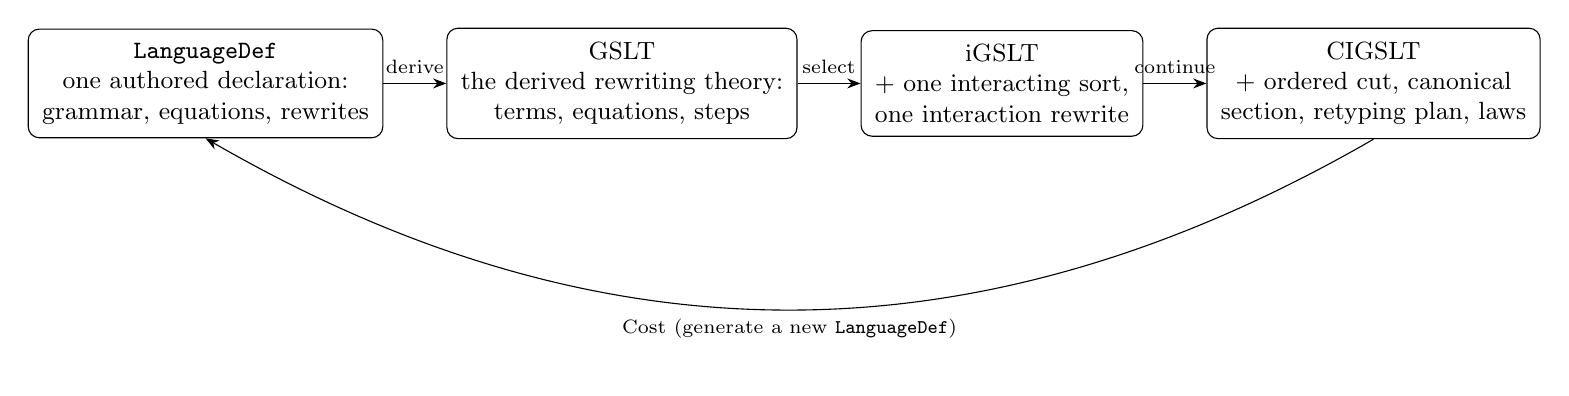
\begin{tikzpicture}[node distance=4mm and 8mm,
  box/.style={draw, rounded corners, align=center, inner sep=5pt,
    font=\small}]
\node[box] (ld) {\code{LanguageDef}\\one authored declaration:\\grammar, equations, rewrites};
\node[box, right=of ld] (gslt) {GSLT\\the derived rewriting theory:\\terms, equations, steps};
\node[box, right=of gslt] (igslt) {iGSLT\\$+$ one interacting sort,\\one interaction rewrite};
\node[box, right=of igslt] (cigslt) {CIGSLT\\$+$ ordered cut, canonical\\section, retyping plan, laws};
\draw[-{Stealth}] (ld) -- (gslt) node[midway,above,font=\scriptsize]{derive};
\draw[-{Stealth}] (gslt) -- (igslt) node[midway,above,font=\scriptsize]{select};
\draw[-{Stealth}] (igslt) -- (cigslt) node[midway,above,font=\scriptsize]{continue};
\draw[-{Stealth}] (cigslt.south) to[out=-150,in=-30]
  node[midway,below,font=\scriptsize]{$\mathrm{Cost}$ (generate a new \code{LanguageDef})} (ld.south);
\end{tikzpicture}
}
\end{center}

\noindent
The loop closes at the left: Cost consumes a continued object and emits a
new \emph{authored-style declaration} --- the generated funded language of
Section~\ref{sec:genfunded} --- which re-enters the same tower.  Nothing
in the tower is hand-written twice; every stage is derived or selected
from the stage before it.

\subsection{Continued interactive GSLTs}

A \emph{generated syntactic labelled transition system} (GSLT) is the
rewriting theory mechanically derived from one authored
\code{LanguageDef}; an \emph{interactive} GSLT (iGSLT) additionally fixes
a validated presentation with one distinguished interacting sort and one
interaction rewrite.  A \emph{continued interactive GSLT} (\code{CIGSLT})
equips an iGSLT with exactly the data Cost needs to fire again:

\begin{itemize}
\item one ordered authored \emph{interaction cut}: the core contact
  constructor, and a program operand and an environment operand, each an
  authored constructor together with its selected \emph{continuation
  position} and continuation schema variable;
\item a \emph{computable contextual open section}: canonicalization on
  every declaration-derived open sorted fiber, retaining sort,
  free-variable context, binder context, and reflective scope
  (Section~\ref{sec:canon});
\item a \emph{continuation retyping plan}: the finite declaration-level
  recipe that sends every constructor except the two selected principals
  to a hereditarily \emph{wrapped} copy, and the two principals to
  \emph{cut-aware base} copies whose continuation parameter alone is
  retyped into the wrapped fiber;
\item closure laws, each a proposition over the plan: every equation and
  every reflective presentation of the source survives the retyping with
  sorted base and wrapped images (\code{EquationsRetypable},
  \code{ReflectivePresentationsRetypable}); the selected redex and
  contractum remain sorted after their continuation positions move to the
  wrapped fiber (\code{RedexRetypable}, \code{Wrappable}); the authored
  envelope around the interaction core is a signature context stable
  under retyping (\code{sourceEnvelopeStable}); every bare-collection
  constructor --- whose label is invisible in raw syntax --- is
  explicitly non-principal (\code{bareCollectionConstructorsWrapped});
  and canonicalization preserves the non-principal typed constructor
  fragment, so normalization can never manufacture an interaction
  principal.
\end{itemize}

The last two laws deserve emphasis because each answers a concrete
soundness hazard.  A bare collection hides its constructor label in the
raw pattern, so a typing derivation chooses its rule non-syntactically;
requiring all such rules to be non-principal makes every hidden choice
harmless \emph{independently of which candidate a derivation picked}.
And requiring the canonicalizer to preserve the non-principal fragment
closes the loop between normalization and interaction: rearranging
authored static structure is allowed, manufacturing a redex is not.

In Lean the object is one structure, reproduced here abridged
(\leanfile{GSLT/LanguageDef/ContinuedCategory.lean}{ContinuedCategory.lean}):

\begin{lstlisting}
structure CIGSLT where
  theory        : IGSLT
  cut           : InteractionCutPresentation theory
  openCanonical : ComputableContextualOpenSection theory
  continuationRetyping : ContinuationRetypingPlan cut
  bareCollectionConstructorsWrapped : ...  -- hidden labels are non-principal
  openCanonicalPreservesWrappedConstructorTyping : ...
  equationsRetypable               : EquationsRetypable continuationRetyping
  reflectivePresentationsRetypable : ...
  sourceEnvelopeStable             : ContinuationStableContext cut ...
  redexRetypable : continuationRetyping.RedexRetypable
  wrappable      : continuationRetyping.Wrappable
\end{lstlisting}

\noindent
Every law is a proposition over \code{(theory, cut, plan)} alone --- a
deliberate design point: the closure obligations of the \emph{generated}
object are statable before that object is fully assembled, which is what
Section~\ref{sec:endofunctor} exploits.

\subsection{Position-sensitive retyping is not a morphism}

The retyping plan is deliberately \emph{not} a uniform signature
morphism, and this is a theorem-shaped fact rather than an
implementation convenience.  The generated language declares base copies
of every source constructor and wrapped copies of the non-principals;
the two principals receive \emph{cut-aware} base copies whose
continuation parameter is wrapped while every other parameter is base.
Consequently no single symbol action covers the retyping: occurrences of
the wrapped sort must map differently at continuation positions than
elsewhere.  The formal development therefore transports typing
derivations along the plan with a dedicated induction
(\code{mapCostStaticGenerated}), stated over exactly
(theory, cut, plan) plus the bare-collection law --- and over nothing
else.  This minimal signature is what makes the construction iterate
without circularity: the generated object inhabits it before the
generated object's own closure laws are discharged. \formalized

\subsection{The generated funded language}
\label{sec:genfunded}

From a \code{CIGSLT} the construction produces the complete funded
language in two stages.  The \emph{continuation signature} is the
generated base/wrapped grammar above.  The \emph{whole language} adds a
small administrative apparatus --- a contact constructor, a signing
wrapper, funding and token-stack constructors --- and exactly one
rewrite, the \emph{whole-redex rule}: the base-mapped source redex,
signed and placed beside a funding stack whose head carries the demanded
signature, contracts in one step to the wrapped contractum beside the
unconsumed stack tail.  The generated source pattern is positively
characterized --- it is literally one explicit contact of a signed redex
with a matching funded stack
(\leanfile{GSLT/LanguageDef/CostInteraction.lean}{CostInteraction.lean},
theorem \code{costWholeRedexSource\_eq}):

\begin{lstlisting}
-- left side of the one generated rewrite
contact( signed( <base-mapped source redex> , $sig ),
         funding( stackCons($sig, $tail) ) )
-- right side
contact( <wrapped source contractum> , funding($tail) )
\end{lstlisting}

\noindent
The rule consumes the stack head and carries the tail variable through
unchanged, and no rule creates a replacement token. \formalized{} Funding is thereby part of the
\emph{grammar and one rewrite} of an ordinary authored-style language ---
not a side condition bolted onto an evaluator --- which is what makes the
output of Cost a candidate input to Cost again.

\subsection{Morphisms and the ordered category}

Continued objects form a category.  A morphism is an iGSLT theory map
that preserves the ordered cut (core contact, both operand constructors,
core pattern, and envelope), reflects the interacting-sort fiber,
preserves and reflects the finite wrapped-constructor closure, and
commutes with canonicalization injectively on canonical keys.  The
forgetful functor to iGSLTs forgets object structure but no morphism
action. \formalized{} On top of this sits the \emph{ordered} category:
canonical keys carry a collision-free structural code, giving every
object a linear order on keys, and ordered morphisms are those whose
key action is monotone.  Exact typed Cost objects
(Section~\ref{sec:canon}) then form an honest full subcategory ---
written \code{CostOneObjects} --- which is the intended domain of strict
$\mathrm{Cost}_1$. \formalized

\section{Typed normalization: a refutation and its repair}
\label{sec:typednorm}

The July development exposed a second incorrect hypothesis, this time in
our own earlier normalization architecture, and the repair reshaped the
whole equational layer.  We record both, because the counterexample is
compiled and the repair is, we believe, the right general discipline for
proof-relevant rewriting over generated languages.

\paragraph{The refutation.} The earlier normalization laws demanded a
global \emph{raw fiber stability}: that every raw equation-equivalence
between patterns in a typed fiber restricts to that fiber.  For the rho
instance this is \emph{false}, and the falsity is witnessed by a
compiled counterexample: a mixed-colour reflective generator whose left
endpoint is typed while its canonical right endpoint is ill-typed.
\refuted{} A raw equivalence endpoint is simply too weak a datum: raw
syntax cannot remember the binder slice that typing carries.

\paragraph{The repair: typed equation carriers.} The equational theory
is now carried at the typed level.  Open patterns in a declaration-derived
fiber carry their typing; the authored equations generate a setoid on
these \emph{typed} carriers; and the two directions between raw and
typed are deliberately asymmetric.  Typed-to-raw erasure is free.
Raw-to-typed lifting exists only edge-wise: one authored contextual
generator step whose \emph{two endpoints are already packaged in the
same typed open fiber} may be injected, and the endpoint certificates
are the entire distinction from the refuted operation, which attempted
to lift an opaque raw path after the fact
(\leanfile{GSLT/LanguageDef/EquationSubstitution.lean}{EquationSubstitution.lean}).
\formalized

\paragraph{Proof-relevant elaboration.} Above the typed carriers sits a
proof-relevant elaboration layer: a cost region tree is a typed
derivation of how a pattern decomposes into coloured static regions, and
normalization is defined on trees, not on raw syntax.  Compilation
chooses a tree but contributes no semantic equation authority; the
executable compact normalizer inherits typed soundness from the
elaboration it erases.  The normalization theorem lands in the typed
open-equation setoid of the exact fiber --- with \emph{no} global raw
fiber-stability hypothesis anywhere in its statement or proof
(\leanfile{GSLT/LanguageDef/CostRegionNormalization.lean}{CostRegionNormalization.lean}).
\formalized

\paragraph{Exact Cost objects.} An object carries \emph{exact} typed
canonical laws (\code{CostOpenCanonicalLaws}) when typed unary
normalization is sound in every fiber, compact normalization is
coherent across elaboration choices, and each authored open-equation
generator is collapsed.  On such objects the normalizer is a computable
section of every typed open fiber: equivalence classes coincide with
canonical representatives, completeness being generated solely from
exact invariance under the authored generators.  These laws are an
object \emph{property} --- membership is semantic, not structural ---
and cut out the full subcategory on which strict $\mathrm{Cost}_1$
lives. \formalized

\section{Cost as an endofunctor: the object-closure programme}
\label{sec:endofunctor}

Iterating Cost means: the generated funded language, with its generated
cut and generated retyping plan, is again a continued object.  The data
triple exists by construction.  The closure laws are theorems to be
proved \emph{generically} --- for every source object --- and this
programme
(\leanfile{GSLT/LanguageDef/CostEndofunctor.lean}{CostEndofunctor.lean})
is now largely discharged:

\begin{itemize}
\item every bare-collection constructor of the generated language is
  non-principal at the next layer (the generated principals never use
  bare collections, by the source laws) \formalized;
\item the generated interaction envelope is stable under the next
  retyping, by transport of the source envelope-stability witness
  \formalized;
\item there is a single declaration-derived typing morphism from the
  complete generated language into the signature that validates the
  next layer (\code{costClosureTyping}), reusable by the equation,
  contractum, and reflective closure proofs \formalized;
\item the generic typed transport along a retyping plan
  (\code{mapCostStaticGenerated}) is stated and proved over the minimal
  non-circular signature described in
  Section~\ref{sec:continued}. \formalized
\end{itemize}

The remaining obligations --- sorted base and wrapped images of the
generated equations, sortedness of the twice-retyped redex and
contractum, reflective-presentation survival, canonical preservation of
the next non-principal fragment, and the contextual strengthening of the
typed canonical section --- are active work; each has an identified
proof route through the theorems above, and none requires new global
hypotheses.  \open{} Two structural facts already shape the endgame:
closure lands on the exact full subcategory (the laws of
Section~\ref{sec:typednorm} must themselves be closed), and the uniform
shortcut is provably unavailable --- the twice-retyped redex cannot be
transported by any single signature morphism, because the declared
cut-aware principal copies disagree with the uniform image at exactly
the two continuation parameters.

\section{Canonical forms and the computable section}
\label{sec:canon}

Signature keys, and every quotient used above, presuppose a
\emph{computable canonical form} for the two static equivalences of the
pure calculus. A canonicalizer $\mathsf{nf}$ must:
\begin{itemize}
\item normalize binders so that alpha-equivalent terms coincide
  (locally nameless or de Bruijn representation);
\item normalize processes and names mutually, with termination measured
  by quote depth;
\item orient the name cancellation $@({*}x) \equiv_N x$ as a directed
  simplification;
\item flatten parallel composition, remove $0$, normalize components
  recursively, and sort them under a proved total order on terms;
\item keep name equivalence and process congruence as \emph{separate}
  sorted relations --- the canonical form respects both without merging
  them into one relation over raw syntax.
\end{itemize}
The obligations are soundness ($\mathsf{nf}(P) \equiv P$), completeness on
the pure carrier
($P \equiv Q \Rightarrow \mathsf{nf}(P) = \mathsf{nf}(Q)$), and
idempotence. \formalized{} The proved carrier consists of patterns without
the optional finite-set extension.  Canonicalization preserves that subtype
and descends by quotient lifting to a computable representative function; the
representative is proved to belong to its original equivalence class.  The
continued-cut presentation now stores this explicit representative carrier
and embedding instead of selecting representatives with
\code{Quotient.out}.

The mathematical key is the canonical form itself. A runtime digest may later
refine it under an explicitly assumed collision-resistance property, and the
formalization never treats a concrete hash function as injective.

In the formal development this section is \emph{contextual and open}: it is
indexed by every declaration-derived open sorted fiber --- free-variable
context, binder context, and reflective scope included --- and additionally
preserves free-variable support, is natural under agreeing recontextualization
of unused entries (exact raw representative equality, not merely contextual
equivalence), and preserves reflective support.  The closed paper-facing
section above is its restriction to the closed interacting fiber.  The typed
Cost normalizer of Section~\ref{sec:typednorm} is held to the same
interface. \formalized{} for the pure section; the contextual strengthening of
the Cost-side section is part of the open endofunctor obligations of
Section~\ref{sec:endofunctor}.

\section{One authored presentation and semantic agreement}

The pure syntax, equations, reflective constructors, and COMM rule are authored
once in the rho language definition.  The derived well-sorted judgments supply
the induction principles for names, processes, and parallel lists.  On that
derived process carrier, reflective substitution compiled from the authored
declaration is proved exactly equal to the independently developed semantic
COMM substitution.  Every supported COMM contractum compiled from the authored
rule is therefore both a step of the GSLT derived from that same declaration
and an agreement point with the established semantic relation. \formalized{}

The restriction to the derived process judgment is essential.  The shared raw
pattern type also contains ill-sorted terms, including quotations placed
directly in process position; no global agreement theorem is claimed for those
terms.  During the proof, this restriction exposed and led to the repair of an
overlapping unary-pattern dispatcher that could descend beneath a quotation.
A regression example now fixes that boundary.

\section{Scoped funded execution refines pure rho}
\label{sec:scoped-refinement}

The raw de Bruijn representation is intentionally larger than the object
language: it can express an index that is outside its enclosing binder, and it
can retain such an index underneath a quotation.  These values are useful as
negative tests, but they are not rho terms.  Following the standard
scope-safe-syntax discipline~\cite{allais-scope-safe}, the funded syntax has a
derived \emph{binder-safe} judgment tailored exactly to pure erasure.  It checks
all syntax observable after erasure; purse surfaces, which the pure projection
removes, are deliberately outside this judgment.  A separate executable
runtime-scope predicate checks every raw field, including purse surfaces, and
public admission requires it together with grammar validity.  Runtime scope is
proved to imply the pure-erasure binder-safe judgment.  A quotation
seals the surrounding binder,
so a term quoted inside a receiver body must already be closed with respect to
that body.  The judgment is derived over the existing cost syntax; it neither
adds a second syntax nor changes COMM.

The refinement result has the usual initialization--preservation--simulation
shape.  First, flattening a binder-safe source term into a funded configuration
preserves binder safety.  Second, every declarative funded step maps a
binder-safe configuration to a binder-safe configuration.  Third, cost
substitution on this fragment agrees, up to the \emph{pure}
\code{StructuralCongruence}, with the established semantic COMM substitution.
The proof uses the pure canonical section and never an equivalence containing
the executable free-Drop rule. \formalized{}

Configuration erasure is defined by quotient lifting over permutation of
funded components, never by selecting a representative with
\code{Quotient.out}.  Each binder-safe \code{CostStep} then erases to one
step of the pure GSLT derived from \code{rhoCalc}.  Induction over declarative
paths gives a rewrite path in that same derived GSLT; its length is exactly the
number of funded events and exactly the length of the path's ordered demand
receipt.  Thus erasure inserts neither administrative reductions nor
executable-Drop reductions. \formalized{}

The executable/declarative commuting edge is also formalized.  Every publicly
admitted budgeted Lean execution yields its occurrence-bearing runtime path, a
same-length declarative funded trace, and a rewrite path of that same length in
the pure GSLT derived from \code{rhoCalc}.  Structural normalization seams
remain explicit; they are not replaced by syntactic equality. \formalized{}

At the parallel boundary, every list of enabled modeled runtime candidates
whose complete endpoint-and-funding source-index family is globally
duplicate-free lifts to a selected runtime wave.  The wave's witnessed source
partition constructs a fixed compatible cost matching, and every permutation
of that matching serializes as an ordinary declarative cost trace.  This is a
theorem about the Lean runtime model under its occurrence-claim postcondition;
it is not a universal theorem that the compiled C implementation satisfies the
postcondition. \formalized{}

The compiled C engine is checked independently by differential execution and
Lean receipt replay, including rejection of tampered receipts.  That evidence
is deliberately not presented as a universal theorem about compiled C.

\section{Provenance and status}

The formalization pins the exact manuscript versions it implements ---
title, date, and content digest recorded alongside the theory --- because
a silently updated source would change the meaning of proved names. The
operative sources are the reflective higher-order calculus paper of
Meredith and Radestock; the graph-enriched Lawvere-theory account of
operational semantics of Stay and Meredith; and the June 2026 versions of
the continued-interactive-GSLT/cost and cost-accounted-rho manuscripts,
whose earlier circulated revisions differ materially and are kept only as
comparison history.

\begin{center}
\begin{tabularx}{\textwidth}{@{}Xll@{}}
\toprule
Item & Section & Status \\
\midrule
COMM-only concrete one-step relation & \S2 & formalized \\
Free drop inert in pure rho (negative theorem) & \S2, \S4 & formalized \\
Runner idiom (one-COMM execution) & \S3 & stated; example-level \\
Execution delta with positive/negative theorems & \S4 & formalized \\
Fixed-element cancellation boundary & \S5(a) & formalized \\
$\mu$ joint-injectivity impossibility & \S5(b) & formalized \\
Parameterized monad laws on funded execution & \S5 & formalized \\
Exact receipt / lossy aggregate factorization & \S5 & formalized \\
Continued category (objects, morphisms, ordered keys) & \S6 & formalized \\
Generated funded language: whole-redex rule, positive shape & \S6 &
  formalized \\
Generic typed transport over (theory, cut, plan) & \S6 & formalized \\
Raw fiber stability for rho & \S7 & counterexample recorded \\
Typed equation carriers; edge-wise raw-to-typed lifting & \S7 & formalized \\
Proof-relevant elaboration; typed normalization soundness & \S7 &
  formalized \\
Exact canonical laws; \code{CostOneObjects} subcategory & \S7 & formalized \\
Endofunctor closure: bare-collection, envelope, closure typing & \S8 &
  formalized \\
Endofunctor closure: remaining object laws & \S8 & open \\
Computable pure canonical form + section & \S9 & formalized \\
Authored COMM compiler agreement with established semantics & \S10 &
  formalized \\
Binder-safe initialization and preservation & \S11 & formalized \\
Funded-step erasure to the LanguageDef-derived pure GSLT & \S11 &
  formalized \\
Runtime and declarative paths to derived pure paths, exact length & \S11 &
  formalized \\
Occurrence-disjoint modeled runtime waves to fixed cost matchings & \S11 &
  formalized \\
Pure/extended and cost-profile execution boundary & \S4 &
  Lean theorems; C differential gate \\
\bottomrule
\end{tabularx}
\end{center}

\begin{thebibliography}{9}

\bibitem{meredith-radestock}
L.~G. Meredith and M.~Radestock.
\newblock A reflective higher-order calculus.
\newblock \emph{Electronic Notes in Theoretical Computer Science},
  141(3):49--67, 2005.

\bibitem{stay-meredith}
M.~Stay and L.~G. Meredith.
\newblock Representing operational semantics with enriched Lawvere
  theories.
\newblock 2017.

\bibitem{cost-manuscripts}
L.~G. Meredith.
\newblock Continued interactive GSLTs and the cost endofunctor: wrapping
  by construction; and Cost accounting for the reflective higher-order
  calculus.
\newblock Manuscripts, June 2026 versions (pinned by digest in the
  repository).

\bibitem{mettail}
F1R3FLY-io.
\newblock \emph{mettail}: a reference implementation family for
  rho-style calculi.
\newblock Open-source repository; used here as a bounded encoding
reference, with its implementation delta recorded in
Section~\ref{sec:ext}.

\bibitem{atkey}
R.~Atkey.
\newblock Parameterised notions of computation.
\newblock \emph{Journal of Functional Programming}, 19(3--4):335--376,
  2009.
\newblock \url{https://bentnib.org/param-notions.html}

\bibitem{katsumata}
S.~Katsumata.
\newblock Parametric effect monads and semantics of effect systems.
\newblock In \emph{Proceedings of POPL}, 2014.
\newblock \url{https://group-mmm.org/~s-katsumata/paper/ppl2014.pdf}

\bibitem{orchard-wadler-eades}
D.~Orchard, P.~Wadler, and H.~Eades~III.
\newblock Unifying graded and parameterised monads.
\newblock In \emph{Proceedings of MSFP}, 2020.
\newblock \url{https://arxiv.org/abs/2001.10274}

\bibitem{allais-scope-safe}
G.~Allais, R.~Atkey, J.~Chapman, C.~McBride, and J.~McKinna.
\newblock A type- and scope-safe universe of syntaxes with binding: their
  semantics and proofs.
\newblock 2021.
\newblock \url{https://arxiv.org/abs/2001.11001}

\end{thebibliography}

\end{document}
